\section{Restricted correspondences and obstructions}\label{sec:corr}
Two integer systems act on the same states: the collective map $C$ and the generative \emph{SELECT-II} edges~\cite{FoundI} $T_N:m\mapsto m(N+1)^2/N$ ($N\mid m$). This section records what can be compared exactly between them. The comparison is graded by levels, and \emph{a level is never inferred from a weaker one}.

\begin{definition}[levels of correspondence]\label{def:levels}
\textbf{L1} (numerical): the two systems relate the same pair of states, or the same ratio $x_m/x_n$. \textbf{L2} (occurrence information): equal initial and final occurrence structures. \textbf{L3} (reduced event records): equal numbers (and, for integers, equal $\sigma$-sequences) of occurrence-changing steps along the two paths. \textbf{L4} (geometric structures): equal realised complexes along the paths. \textbf{L5} (dynamical intertwining): a map conjugating the two dynamics. The hierarchy runs L1 $\to$ L2 $\to$ L3 $\to$ L4 $\to$ L5 in increasing strength; each level is tested on its own.
\end{definition}

\subsection{Transport along a SELECT-II edge}
\begin{theorem}[box transport, B2-T2]\label{thm:B2T2}
Let $m\xrightarrow{N}m'=m(N+1)^2/N$ with $N\mid m$, and let $p$ be a prime, $n=v_p(N)$, $w=v_p(N+1)$ (at most one of $n,w$ is non-zero). Then $q_p(m')=q_p(m)+w$ if $p\nmid N$, and $q_p(m')=q_p(m)-l_p$ if $p\mid N$, where $l_p=\lfloor n/2\rfloor$ if $v_p(m)$ is odd and $l_p=\lceil n/2\rceil$ if $v_p(m)$ is even. Consequently $\sigma(m')=\sigma(m)(N+1)/c$ with $c=\prod_{p\mid N}p^{l_p}\le N$.
\end{theorem}
\prov{CW-0396}{B2-T2}{PROVED}{FULL}
\begin{proof}
$v_p(m')=v_p(m)+2w-n$. For $p\nmid N$ ($n=0$) the change $2w$ is even, so $\lfloor v_p/2\rfloor$ increases by $w$. For $p\mid N$ ($w=0$), put $e=v_p(m)\ge n$: $\lfloor(e-n)/2\rfloor=\lfloor e/2\rfloor-\lfloor n/2\rfloor$ if $e$ is odd and $\lfloor e/2\rfloor-\lceil n/2\rceil$ if $e$ is even. Multiplying over primes, $\prod_{p\mid N+1}p^{w}=N+1$ and $c\le\prod p^{n}=N$. \qedhere
\end{proof}
\begin{theorem}[gain--loss balance, B2-T3]\label{thm:B2T3}
For a history with labels $N_1,\dots,N_r$ put $G_p=\sum_iv_p(N_i+1)$ and let $\Lambda_p$ be the total decrease of $q_p$ over the steps with $p\mid N_i$. Then $q_p(\mathrm{end})-q_p(\mathrm{start})=G_p-\Lambda_p$, so the loss budget $\Lambda_p$ is determined by the content and the endpoints, not by the order. If two admissible blocks $u,v$ from the same state have equal endpoints, then
\[
\Lambda_p(u)-\Lambda_p(v)=\tfrac12\big(H_p(u)-H_p(v)\big),\qquad H_p=\sum_iv_p(N_i)\ \text{(denominator content).}
\]
\end{theorem}
\prov{CW-0397}{B2-T3}{PROVED}{FULL}
\begin{proof}
Telescope \cref{thm:B2T2}. The multiplier of a history is $\prod_i(N_i+1)^2/N_i$; equal endpoints from the same state force $2G_p(u)-H_p(u)=2G_p(v)-H_p(v)$ for every $p$, and substituting $G_p=\Delta q_p+\Lambda_p$ (with $\Delta q_p$ equal for $u$ and $v$) gives the relation. \qedhere
\end{proof}
\begin{theorem}[parity conservation, restricted]\label{thm:B2T4}
Let every label of a history satisfy $v_p(N)\le1$ and let $c$ be the number of labels divisible by $p$. Then the parity of $v_p$ flips at each of these $c$ edges and is unchanged at the others. The $p$-edges therefore see the parities $\pi,\pi+1,\pi,\dots$ in order ($\pi$ the parity of $v_p$ at the start), and the loss steps for $p$ are those that see an even parity: their number is $\lceil c/2\rceil$ if $\pi$ is even and $\lfloor c/2\rfloor$ if $\pi$ is odd, whatever the order of the labels. Orderings only permute when the losses occur. No claim is made outside $v_p(N)\le1$.
\end{theorem}
\prov{CW-0398}{B2-T4}{PROVED-SCOPED}{FULL}
\begin{proof}
For $p\mid N$ with $n=v_p(N)=1$ we have $w=0$ and $v_p(m')=v_p(m)-1$, so the parity flips; for $p\nmid N$, $v_p(m')=v_p(m)+2w$, so it does not. By \cref{thm:B2T2}, $l_p=\lfloor1/2\rfloor=0$ if $v_p(m)$ is odd and $l_p=\lceil1/2\rceil=1$ if $v_p(m)$ is even; a loss for $p$ is therefore a $p$-edge taken at even $v_p(m)$. The alternation of parities gives the count. \qedhere
\end{proof}
\begin{remark}[correction of wording]
The inherited summary describes the loss step as the one with $v_p(m)$ odd; by \cref{thm:B2T2} it is the one with $v_p(m)$ even (for $n=1$ an odd exponent loses nothing). The parity-flip conclusion is unaffected.
\end{remark}

\subsection{Rigid relations and one-step obstructions}
\begin{proposition}[one-step obstruction]\label{prop:onestep}
For every state $x$ with $D(x)\ne\emptyset$, $1<C(x)/x\le2$, whereas $T_N(x)/x=R(N):=(N+1)^2/N\ge4$ for every $N\ge1$. Hence $C(x)\ne T_N(x)$ for all $N$: one collective step is never a SELECT-II edge.
\end{proposition}
\begin{proof}
$C(x)/x=1+L^2/(ah)$ and $L^2\mid a$, $h\ge1$ give $L^2/(ah)\le1$. $R(N)=N+2+1/N\ge4$ with equality iff $N=1$. \qedhere
\end{proof}
\begin{theorem}[snapshot relation, B-T12]\label{thm:BT12}
On the rigid domain (\cref{thm:B2T6}, $t\in\{1,2,3\}$, $G=1$) $C^3(x)=4x=T_1(x)$. This relation holds at the snapshots $n\equiv0\pmod3$ only: by \cref{prop:onestep} no single collective step equals a SELECT-II edge, so the relation is \emph{not} a conjugacy of the two systems (no L5).
\end{theorem}
\prov{CW-0394}{B-T12}{PROVED}{FULL}
\begin{proof}
\Cref{thm:B2T6} and $T_1(x)=4x$; the second part is \cref{prop:onestep}. The identity $C^3=4x$ was also checked on $90$ integers of the rigid domain (\stat{finite-exact}). \qedhere
\end{proof}
\begin{theorem}[rigid event correspondence, B2-T10]\label{thm:B2T10}
Let $x=t\sigma^2$, $t\in\{1,2,3\}$, $\sigma$ even. The collective orbit passes from $x$ to $C^3(x)=4x$ with reduced $\sigma$-sequence $(\sigma,2\sigma)$, one birth event and $\tau(\mu)$ new occurrences, $\sigma=2^a\mu$, $\mu$ odd; the single edge $T_1:x\mapsto4x$ has the same $\sigma$-sequence, one birth event and the same number $\tau(\mu)$ of new occurrences. L3 holds. L4 holds at the integer endpoints by \cref{thm:B2T1}; L5 does not (\cref{thm:BT12}).
\end{theorem}
\prov{CW-0404}{B2-T10}{PROVED}{FULL}
\begin{proof}
For $\sigma$ even $G=1$, so \cref{thm:B2T6} applies: the carry occurs at the third step ($t=3\to1$, $u=2$) and $D$ changes only there, with $\tau(2\sigma)-\tau(\sigma)=\tau(\mu)$ new elements (\cref{thm:B2T8}). The edge $T_1$ sends $\sigma\to2\sigma$ ($c=1$, $N+1=2$) with the same count. By \cref{thm:B2T1} the box record of an integer is a function of $\sigma$. \qedhere
\end{proof}
\begin{theorem}[a coincidence family, B2-T12]\label{thm:B2T12}
Let $N=2^a-1$ be squarefree ($a\ge2$), $s$ even, $x=Ns^2$. Then $C^k(x)=T_N(x)=(2^as)^2$ with $k=1+3a/2$ for $a$ even and $k=1+2+3(a-1)/2$ for $a$ odd: $k$ collective steps against exactly one SELECT-II event.
\end{theorem}
\prov{CW-0406}{B2-T12}{PROVED}{FULL}
\begin{proof}
$N$ squarefree gives $\sigma(x)=s$, $t=N$, and $G=1$ since $s$ is even. $T_N(x)=x(N+1)^2/N=(2^as)^2$. For $a$ even, $t+1=2^a$ is a square: $t\to1$, $\sigma\to2^{a/2}s$ in one step; each rigid period $(1,2,3)$ takes three steps and doubles $\sigma$, and $a/2$ periods give $\sigma=2^as$ with $t=1$: $k=1+3a/2$. For $a$ odd, $\sqf(2^a)=2$: $t\to2$, $\sigma\to2^{(a-1)/2}s$; two more steps ($t=2\to3\to1$) double $\sigma$; $(a-1)/2$ further periods are needed: $k=1+2+3(a-1)/2$. \qedhere
\end{proof}
\begin{remark}[finite-exact]
Verified for $a=2,\dots,5$ and $s\in\{2,4,6,8,10\}$ ($k=4,6,7,9$) with the engine; a scan of $x<4000$ in the source found all single-edge coincidences with $N+1\in\{2^a,3\cdot2^a\}$; completeness is \stat{open} and not claimed.
\end{remark}
\begin{theorem}[scaling obstruction, B2-T13]\label{thm:B2T13}
(a) $R(N)=(N+1)^2/N$ is an integer iff $N=1$ (then $R=4$). (b) The multiplier $9$ of the $G=11$ tower is not $R(N)$ for any integer $N$ ($R(N)=9\iff N^2-7N+1=0$, no integer root), and it is not a product of two or more factors $R(N_i)$, since each factor is $\ge4$ and such a product is $\ge16$. (c) The multiplier $900$ of the $\ell=29$ example is not $R(N)$ for any integer $N$.
\end{theorem}
\prov{CW-0407}{B2-T13}{PROVED}{FULL}
\begin{proof}
(a) $\gcd(N,(N+1)^2)=1$, so $R(N)$ is reduced with denominator $N$. (b) $(N+1)^2=9N$ is $N^2-7N+1=0$, with discriminant $45$, not a square; the product bound follows from $R(N)\ge4$ (as $R(N)=N+2+1/N$). (c) $(N+1)^2=900N$ is $N^2-898N+1=0$ with discriminant $898^2-4=806{,}400=896\cdot30^2$, and $896=2^7\cdot7$ is not a square. \qedhere
\end{proof}
\Cref{fig:hierarchy} summarises the hierarchy of levels and the scaling obstruction.
\begin{figure}[tbp]\centering
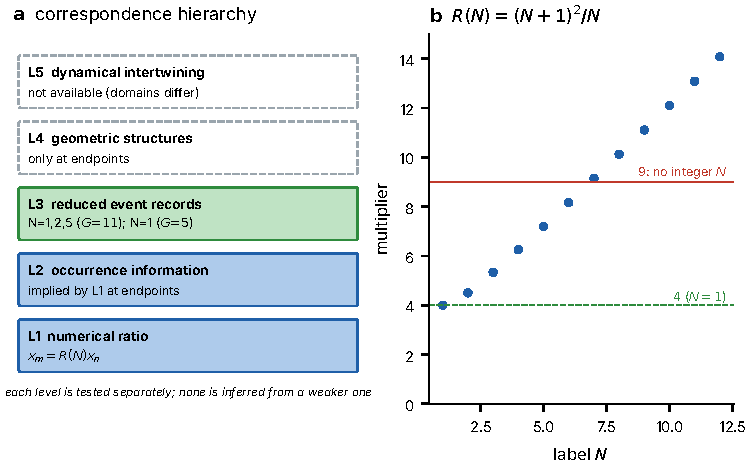
\includegraphics[width=\textwidth]{fig26_hierarchy_obstruction}
\caption{\textbf{The hierarchy and the scaling obstruction (schematic left; exact right).} (a) Levels of correspondence L1--L5 with what is established: L3 for the formal multipliers $N=1,2,5$ ($G=11$) and $N=1$ ($G=5$) at the event level; L4 only at endpoints; L5 not available. The diagram is schematic and each level is tested separately. (b) $R(N)=(N+1)^2/N$ for $N=1,\dots,12$; the integer value $4$ occurs only at $N=1$ and $9$ occurs for no integer $N$ (proved by \cref{thm:B2T13}).}\label{fig:hierarchy}
\end{figure}

\subsection{Formal multipliers on the two towers}
\begin{theorem}[classification of multiplier coincidences, R3-T7]\label{thm:R3T7}
Write the iterates of a tower as $x_n=u\,\rho^{2a}x_0$ with $u\in[1,P]$ ($(P,\rho^2)=(8,9)$ for $G=11$, $(3,4)$ for $G=5$). A pair $n<m$ has $x_m/x_n=R(N)$ for an integer $N$ exactly in the following cases ($x_m/x_n=\rho^{2a}v/u$, $a$ the number of periods crossed, $u,v\in[1,P]$):
\begin{enumerate}[label=(\alph*),itemsep=1pt]
\item $G=11$: $N=1$, $(u,a,v)\in\{(1,0,4),(2,0,8)\}$ (ratio $4$); $N=2$, $(u,a,v)=(2g,1,g)$, $g=1,\dots,4$ (ratio $9/2$); $N=5$, $(5,1,4)$ (ratio $36/5$); $N=8$, $(8,2,1)$ (ratio $81/8$). No other pair has a SELECT-II ratio.
\item $G=5$: $N=1$, $(u,1,u)$ (ratio $4$, a full period); $N=3$, $(3,2,1)$ (ratio $16/3$).
\end{enumerate}
At the event level, with L3 meaning that the number of occurrence-changing steps along the collective segment, which is $a$, equals that of the formal edge, which is $1$ if $D(x_n)\ne D(x_m)$ and $0$ otherwise (that is, $[a\ge1]$): L3 holds for $N=1,2,5$ ($G=11$; for $N=1$ both counts are $0$: the formal $T_1$ is \emph{silent} on these rational states) and for $N=1$ ($G=5$); L3 fails, although L1 holds, for $N=8$ ($G=11$; $a=2$ against $1$) and for $N=3$ ($G=5$; $a=2$ against $1$). The full-period multiplier is $4=R(1)$ for $G=5$ and $9$ for $G=11$, which is not of the form $R(N)$ (\cref{thm:B2T13}).
\end{theorem}
\prov{CW-0422}{R3-T7}{PROVED}{FULL}
\begin{proof}
By \cref{thm:R3T5bp,thm:R3T5c}, $x_{Pk+j}=(j+1)\rho^{2k}x_0$ for $0\le j<P$. Write $x_n=u\rho^{2a_n}x_0$, $x_m=v\rho^{2a_m}x_0$ with $a=a_m-a_n$. The equation $\rho^{2a}v/u=(N+1)^2/N$ is $N\rho^{2a}v=u(N+1)^2$. As $\gcd(N,N+1)=1$, $N\mid u$, so $N\le P$ and $u=Nw$ with $\rho^{2a}v=w(N+1)^2$, $1\le v\le P$, $1\le w\le\lfloor P/N\rfloor$. For $G=11$ ($P=8$, $\rho^2=9$) one checks $N=1,\dots,8$: $9^av=w(N+1)^2$ has the solutions listed (e.g.\ $N=2$: $9^av=9w$ forces $a=1$, $v=w$; $N=8$: $9^av=81$ forces $a=2$, $v=1$; $N=3,4,6,7$ have none because $16w,25w,49,64$ are not of the form $9^av$ with $1\le v\le8$), and similarly for $G=5$ ($P=3$, $\rho^2=4$, $N\le3$). Events: $D$ changes exactly at the steps $x_{Pk}$, $k\ge1$ (\cref{thm:R3T5bp,thm:R3T5c}), so the collective segment from $x_n$ to $x_m$ crosses exactly $a$ of them, and $D(x_n)\ne D(x_m)$ iff $a\ge1$. \qedhere
\end{proof}
\begin{remark}[finite-exact check; phase shift]
Brute force over the first $41$ iterates ($G=11$) and $19$ iterates ($G=5$) found exactly these cases, with $10,17,4,4$ pairs for $N=1,2,5,8$ ($G=11$) and $16,5$ pairs for $N=1,3$ ($G=5$), and the event counts $0,1,1,2$ and $1,2$ respectively (\stat{finite-exact}). A phase-shifted correspondence holds on the $G=11$ tower: $C^{8-g}(2gS^2/11)=\tfrac92\cdot2gS^2/11$ for $g=1,\dots,4$ (the formal edge $N=2$, $R(2)=9/2$), verified for $S=S_0$; the multiplier $9$ itself is not representable. The $\sigma$-track step of one period ($L:S_k\to3S_k$) is realised by a genuine integer edge ($m=2S_k^2\xrightarrow{2}9S_k^2$) with multiplier $9/2$ rather than $9$. These are statements about L1--L3 only; no L4 beyond endpoints and no L5 is claimed.
\end{remark}

\subsection{Corrected block and cited results}
\begin{proposition}[the SELECT-II block, B2-T14 (split)]\label{prop:B2T14}
(i) \emph{Common carrier} (proved): the generative edge acts on $\sigma$ by $\sigma\mapsto\sigma(N+1)/c$ (\cref{thm:B2T2}), and the collective regime-I carry by $\sigma\mapsto\sigma u$ (\cref{thm:B2T6}); both are rules on the same object, but with unrelated multipliers, meeting only in the rigid case, the coincidence family and the $N=1$ obstruction. (ii) \emph{Level 3 $\Rightarrow$ level 4 for integers} (proved): the box record of an integer state is a function of $\sigma$ (\cref{thm:B2T1}), so equal $\sigma$-sequences give equal geometric records. (iii) \emph{Loss-budget blindness} (\stat{cited}, finite-exact): the geometric events of a history do not see the loss budget $\Lambda$; this part rests on inherited computations and is not re-derived.
\end{proposition}
\prov{CW-0408}{B2-T14}{PROVED}{SPLIT}
\begin{remark}[cited]
The following inherited records are \stat{cited}, with ownership as in Appendix~\ref{app:crosswalk}: B2-T5 (mixed-index forcing, proved for contents $2^\alpha3^\beta$ and open for $k>2$ primes), B2-T11 (birth-endpoint classification $x_m=4^jx_n$; finite-exact on $16{,}028$ pairs, not re-run), and, from Paper~II~\cite{PaperII}, R3-T3, R3-T3$'$, R3-T4 and the obstruction A4-T7, discussed below.
\end{remark}
\prov{CW-0399}{B2-T5}{MIXED}{CITED}
\prov{CW-0405}{B2-T11}{PROVED}{CITED}
\prov{CW-0413}{R3-T3}{PROVED}{CITED}
\prov{CW-0414}{R3-T3'}{FINITE-EXACT}{CITED}
\prov{CW-0415}{R3-T4}{PROVED-SCOPED}{CITED}
\begin{proposition}[obstruction to identifying histories with orbits, A4-T7; cited from Paper~II]\label{prop:A4T7}
The move complex of an integer state is contractible (\cref{thm:B2T1}), whereas the history complexes of Paper~II between integer endpoints have two or three components in the cases studied there; consequently no identification of the two kinds of complex is available, and no map between them is claimed. The connection beyond this obstruction is \stat{open}.
\end{proposition}
\prov{CW-0436}{A4-T7}{MIXED}{CITED}
\begin{remark}[no universal correspondence]
Nothing in this section establishes a universal law relating the two systems. What is exact: the transport formulas, the one-step and scaling obstructions, the rigid relation at snapshots, one coincidence family and the classification on two towers. The strongest levels are not inferred from the weaker ones.
\end{remark}
